\chapter{Future work}
\label{chp:futurework} 

\section{Risk}
In our model we used an additive risk parameter, meaning that each connection to a non-insured node adds a fixed negative value $r$ to the node's utility. It is reasonable to assume that the probability of failure increases if a node accepts more and more non-insured nodes. However, whether the risk parameter increases according to an additive distribution is difficult to confirm. Hence the decision of using additive risk was take due to the simplicity of the function and the fact that we do not know for sure how the distribution actually looks like. The probability might as well be multiplicative, exponential or logarithmic. Although it is highly uncertain, we believe that the risk parameter will follow an exponential distribution similar to the one in equation \ref{eq:distributionFunction}.

\begin{equation}
    F(x;\lambda)= 
\begin{cases}
    1-e^{-\lambda x} ,& \text{if } x \geq 0\\
   0,& \text{if }  x<0\\
    
    
\end{cases}
\label{eq:distributionFunction}
\end{equation}



\begin{figure}[h]
\centering
  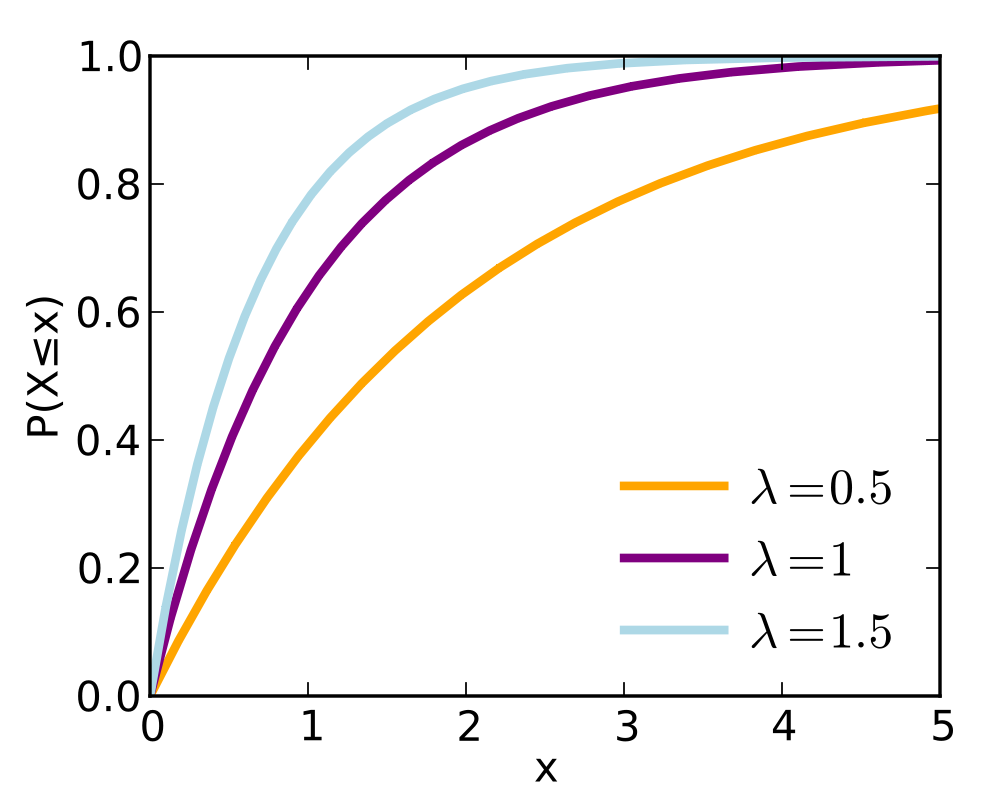
\includegraphics[width=0.5\linewidth]{../Figures/exponentialFunction.png}
  \caption{\label{fig:exponentialFunction} Figure showing the distribution of the equation \ref{eq:distributionFunction}. }
\end{figure}

When $\lambda$ have a value around 0.5, we get a curve \ref{fig:exponentialFunction} which captures how we believe the risk in a network will increase as more non-insured nodes are added. We believe that if one have a growing network consisting of insured nodes only, the first non-insured node added will contribute more risk than the consecutive non-insured nodes. When the 2.nd and 3.rd and so on, node are added there are already a probability that the network will be infected. It reasonable to believe that the overall risk wont increase additive, but at a lower rate. The risk added for each new non-insured node will decrease. Hence we believe that the accentual risk parameter will follow a exponential distribution. 

read more in the paper: Uncertainty in Interdependent Security Games